
\chapter{Test for Disequilibrium}

To achieve this aim I have designed a Likelihood Ratio Test (LRT). The predominant method for examining aspects of sequences' evolution is through the use of \glspl{Substitution model}. \Gls{Maximum Likelihood} methods allow for measuring the support for a hypothesis, (in this case, a \gls{model}), given some data. Whether one hypothesis is better supported than another can be evaluated by using an LRT. Two models fundamental for my LRT are General Nucleotide (GN) and General Nucleotide Stationary (GNS). Their point of difference is that the parameters of a GNS rate matrix must satisfy $\pi\mathbf{Q}=0$, i.e., the process is constrained to be stationary (and thus in equilibrium). Consider an LRT in which GNS is the null and GN is the alternate. If we reject the null, we may conclude that the sequences are more likely to have been generated by a process which is not yet stationary, as this is the only component unique to the alternate.

An LRT as described above is too naive for my objective to test for equilibrium in a single lineage. For a model to be \gls{identifiable} requires an alignment of at least three sequences \cite{Chang1996FullConsistency}. Consequently, a significant result for such an LRT will not reveal which of the taxa is causing the rejection of the null. To test for disequilibrium in a single \gls{edge} requires  modelling a continuous-time process on the edge of interest (herein the foreground edge) and assuming discrete-time processes for the other edges (herein the background edges) \cite{Verbyla2013TheSubstitution}. A discrete-time process is more general (fewer assumptions) than even the GN, making it the ideal background. 

Using mixed discrete- and continuous-time Markov processes, I can test for disequilibrium on a single edge. For such an LRT, the foreground edge assumes GNS for the null, and GN for the alternate. Both hypotheses assume a Barry and Hartigan (BH) model, the most commonly implemented discrete-time process, for the background edges. The modelling of the foreground edge, set apart by the assumption of stationarity, is the only point of difference between hypotheses. For this LRT, a rejection of the null means that the foreground edge was described significantly better with a non-stationary process. Such a result suggests disequilibrium precisely in the foreground edge. Put explicitly, the test will be between the following hypotheses:\\ $\mathbf{H_0}$: the foreground evolved according to the \textbf{GNS}, the background according to BH. \\ $\mathbf{H_1}$: the foreground evolved according to the \textbf{GN}, the background according to BH.\\
\noindent Herein all model fits assume mixed discrete- and continuous-time Markov processes, and a BH process is always assumed for the background edges. For brevity, I will refer to a model by the process assumed on the foreground edge.

\begin{figure}[htbp]
\centering
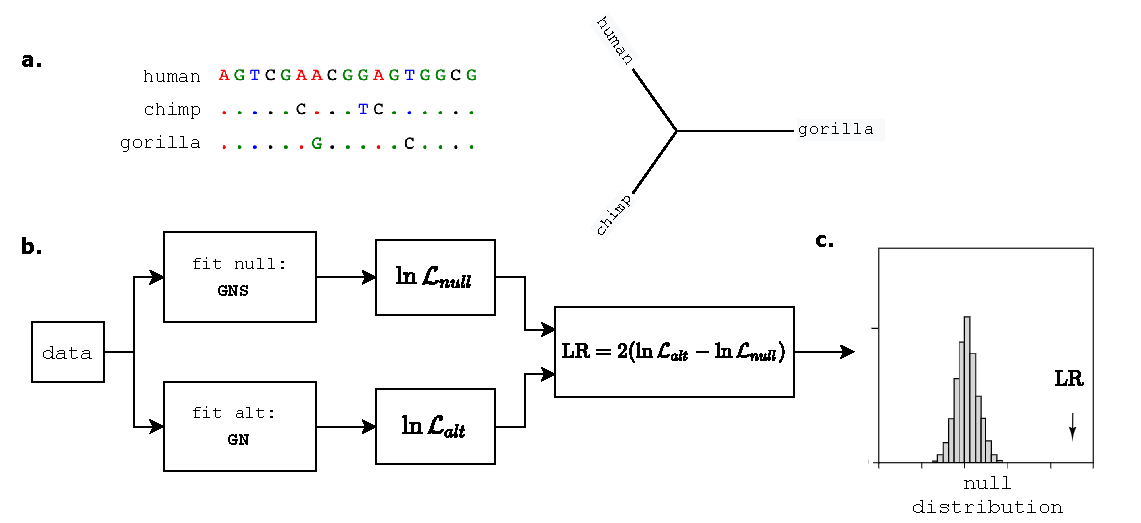
\includegraphics[width=\textwidth]{figures/diagrams/LRT.pdf}
\caption{\textbf{Likelihood Ratio Test.} \textbf{a}, The data: an alignment of orthologous sequences for human, chimp and gorilla, and a phylogenetic tree indicating the relationship between taxa. \textbf{b}, A LRT comparing substitution models, GNS is the null and GN is the alternate. The log-likelihood ($\ln\mathcal{L}$) for each model is obtained via fitting. The likelihood ratio (LR), is the ratio of the $\ln\mathcal{L}$ of the two models. \textbf{c}, the LR statistic is compared to the null distribution. In this case the statistic exceeds the distribution of values we would expect if the null was true, we would thus conclude that process is described significantly better with the alternate (GN) process.}
\label{fig:lrt}
\end{figure}